\chapter{Basic principles of \acs{rfid}} \label{chapter:rfidprinciples}

\section{Contextualization} \label{sec:contextualization}

The concept of identification using \ac{rf} dates back to the late 1930s.
By this time, the primitive biplanes made of wood and fabric used in Word War I, had evolved to all-metal monoplanes. They were capable of carrying heavy quantities of explosives and travel at hundreds of kilometers per hour, making the conventional method of visual identification of incoming aircrafts obsolete.
To counteract this issue, nations invested in research and development that culminated in the development of the microwave radar.
By the time of the World War II, both fronts were using radar technologies to detect approaching planes. 
Still, the problem of identifying allied aircrafts from enemie ones, remained~\footnote{The attack at Pearl Harbor in $1941$ was possible due to a mistaken assignment of incoming Japanese aircraft to an unrelated \ac{us} bomber flight.}.
The German aircraft force, \emph{Luftwaffe}, observed that as pilots rolled their planes, it would change the radio signal reflected back. With this ingeniously simple maneuver, they were capable of discriminate allied aircrafts, being roughly the first \ac{rfid} passive application.~\cite{dobkinRFRFIDSecond2012}

It was soon later that Watson-Watt, under a British project, developed the first active \ac{rfid} application to be used in \ac{iff} systems. An active \ac{rf} transmitter was attached to British planes, which on receiving radar signals from base stations, broadcasted a signal identifying the aircraft as allied.~\cite{HistoryRFIDTechnology}

% This established the core concept of today's systems that make this dissertation possible - the over the air identification of transponders~\footnote{a device that, upon receiving a signal, emits a different signal in response}.

The technology kept advancing through the 1950s and 1960s, mainly in the academic field, but with private companies starting to commercialize anti-theft systems based on 1-bit transponders~\footnote{a simple inductive RC resonant circuit that detects transponders in field by changes in the reader coil voltage~\cite{andreventuradacruzmarnotozuqueteIdentificacaoPorRFID2018}}.

In the 1970s the first \ac{rfid} patents were registered, namely, active tag with rewritable memory and a passive transponder for door lockers. It was during this time that the \ac{us} National Laboratory of Los Alamos was commissioned, by the Energy Department, to develop a tracking system for nuclear materials. The system revolved around transponders in trucks that would transmit information to readers at the gates of secure facilities. The Agricultural Department also requested Los Alamos for an animal tracking system, which was designed in the \ac{uhf} band with passive transponders, marking the beginning of the \acs{uhf}~\acs{rfid} technology. These systems were also transposed by the same engineers to automated toll payment systems in the private industry~\cite{landtHistoryRFID2005, HistoryRFIDTechnology,casierAnalogCircuitDesign2011}.

In the 1980s, the development of the personal computer and technology promises, fueled an upsurge in investment, with private industries wagering in \ac{rfid}.
By the 1990s, deployments of \ac{rfid} systems had grown significantly. The necessity of compatibility and interaction between proprietary systems rose, being established the first industry standards. 

The 2000s followed the same maturation process with slow adoption in the late part of the decade. 
Despite the interest presented by retail giants like Wal-Mart, and investment by the \ac{dod}, compromises created by the \ac{rfid} industry did not justify the commitment to the technology. The high cost for investment, technical performance difficulties, conflicting standards, security issues and privacy concerns made the investment unappealing~\cite{RFIDAdoptionStalls}. 
Companies had to strangle \ac{rnd} resources due to inexistent tools and complex implementations. Resources required to develop marketing and sales tools, which truly utilize the \ac{rfid} infrastructure to increase revenue, had to be allocated to deploy \ac{rfid} systems.
Devise economic strategies for suppliers to transit to \ac{rfid} also seemed to be a problem, since many ordinary companies don't have \ac{rnd} resources at all to begin with~\cite{gaudinSuppliersGainFailed2008}.
Another big issue was the standardization of coding schemes in \ac{rf} tags. The fight for dominance in the \acs{uhf}~\acs{rfid} market led to multiple coding standards and protocols that made inter-operation among vendor and suppliers infeasible, if not impossible.

In the last decade, despite the advancements in the industry and adoption by big apparel retailers like Zara, Decathlon and Marks \& Spencer~\cite{RFIDRetailApparel}, there are issues that inhibit wide-scale adoption of \acs{uhf}~\acs{rfid}. These problems will be further discussed in chapter two of this dissertation.

\section{\ac{rfid} System}

% Reader notes:
% Eu:   talk about the range denomination for systems? close range, long range, ...
%       maybe talk about read range dependence of things (see slides on UHF) - pass the practical considerations section to here as a subsection

\ac{rfid} is an identification technology that uses radio waves or electro-magnetic fields to automatically identify physical objects and collect data about them.

Generally, \ac{rfid} solutions start with a radio device called tag or transponder. The tag is attached to the object that needs to be identified. When such a object is presented in front of an antenna connected to a suitable \ac{rfid} reader, the tag transmits data to the reader via the reader antenna. The reader then forwards the information through a communication channel to a software application running on a computer.

\begin{figure}[]
    \centering
    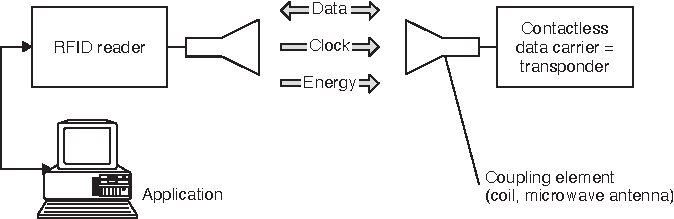
\includegraphics[width=0.8\textwidth]{./figs/02-state-of-the-art/rfid_system.pdf}
    \caption[\ac{rfid} system]{\ac{rfid} system~\cite{finkenzellerRFIDHandbookFundamentals2003}}
    \label{fig:rfidsystem}
\end{figure}

\subsection{Components}

An \ac{rfid} system is a collection of components that implement an \ac{rfid} solution~\cite{lahiriRFIDSourcebook2005}.
Different references present different descriptions of \ac{rfid} systems. Many specify where and which components should be implemented.
The fact is, depending on the use case and requirements, these components can be implemented in different physical places or not implemented at all. With the current paradigm of \ac{iot}, machine learning and cloud computing, the discrimination of these components is even more difficult to establish. It is naive and intricate to predict what \ac{rfid} system architecture will be like in the next few years.

The component description of \ac{rfid} systems can be simplified to three physical blocks: \emph{Tag} (or transponder) which is attached to the physical object to be identified, and is responsible for storing and transmitting appropriate data about the object; \emph{Reader} and \emph{Reader antenna} which interacts with transponders to read and write data; and \emph{Back-end system} which encompasses all kinds of hardware and software components that are separated from the reader and support back-end infrastructures and business logic of a system.

From these, all components described in the literature can be specified and clearly added to one of the blocks.
Other prevalent components used in \ac{rfid} systems are:

\begin{description}
    \item[Controller] is an interface that allows an external entity to communicate with and control the reader's functions and devices connected to it.
    \item[Sensor, actuator and annunciator] are optional components used for external input and output of the system.
    \item[Client Applications] is a term for all hardware and software components that are separated from the reader device (e.g.\ middleware, point-of-sale terminals, etc.)
    \item[Communication infrastructure] is the wired and/or wireless network, or serial connection infrastructure needed to connect the previously listed components
\end{description}

%\subsection{Advantages and Limitations}
%\subsection{Performance factors}
% read range dependance of transmitted power, ... ..

A run through the specificities of most of the components will be done in the following sections.

\section{\acl{em} Concepts} \label{sec:em}

% Readers Notes:
% - Edgar: no inicio parece que as regions são completamente separadas e só nas boundaries é que se percebe que é uma cena progressiva. Ver se re-radiating é uma cena "valida" ou arranjar uma melhor forma de dizer 
% - Eu: rever com o livro RFID Handbook pag. 102, melhorar a escrita, referenciar no texto as imagens e tabelas

Before presenting the intrinsics around \ac{rfid} system components, a basic expertise in \ac{em} concepts is paramount.
Designing well performant systems requires a good understanding of electromagnetism fundaments and its peculiarities.

Like other wireless technologies, \ac{rfid} uses \acp{emf} or \acp{emw} as interface to transmit information back and forward between reader and transponder.
Engineers have to grasp how \acp{emf} and \acp{emw} behave within distance to the reader antenna, how materials in tagged objects can interfere with \ac{rf} signals, how unaccounted poor \ac{rf} environments can compromise deployment of \ac{rfid} systems, to say a few.

An \ac{emf} is the phenomenon produced by moving electric charges. It can be described through Maxwell's equations and mathematical abstracted as a combination of an electric field and a magnetic field that interact with each other and their surroundings.

The behavior of the fields changes as the distance from the source increases and are usually defined as two main regions: \emph{near-field} and \emph{far-field}. These regions separate \ac{rfid} technologies in two very concrete operational groups. In reality, boundaries are not precisely defined, since the regions change their behavior in a progressive manner. The rough discrimination between regions in \ac{rfid} exist to separate mutual coupling and radiation based technologies. 

\subsection{\emph{Near-field}}

\emph{Near-field} manifests from the electric and magnetic fields near the charges and current that directly produced them. It is the region where phenomena like \ac{em} induction and electrostatic occur.
This field can be further split in two regions: reactive \emph{near-field} and radiative \emph{near-field}.

%Due to the variation of the electric rotational field, a magnetic field with closed field lines occurs in space, called rotational field.
%It surrounds the electric field and itself varies over time thus generating another electric field.
%Due to the mutual dependance of the time varying fields there is a chain effect of electric and magnetic fields in space~\cite{finkenzellerRFIDHandbookFundamentals2003}. 

Is in the reactive region that \emph{near-field} \ac{rfid} technologies are defined for. It is the closest to the transmitting antenna and is characterized by non-radiative behaviors. In this region, if the energy is not absorbed by a receiver, self-capacitance and self-inductive effects cause the antenna to store energy very near its surface. When electrons from a nearby conductor are placed in this region, reactive \emph{near-field} energy is transferred to them, resulting in an energy drain on the transmitter by a change in the impedance viewed by the reader~\cite{finkenzellerRFIDHandbookFundamentals2003, balanisAntennaTheoryAnalysis2005}.

In the radiative \emph{near-field}, i.e.\ Fresnel region, the back-coupling of the fields becomes out of phase with the antenna signal, and thus cannot efficiently return inductive or capacitive energy from antenna currents or charges.
In this region conductive objects, such as metal structures, can behave as antennas by inductively receiving and then ``re-radiating'' some of the energy~\cite{ElectromagneticRadiationField}.

The power of the field differers between field components with the distance~($d$) from the antenna. The magnetic field strength is proportional to $1/d^3$ and the electric to $1/d^2$. The \emph{near-field} components are quite powerful but usually only suited for close range \ac{rfid} technologies due to the rapid fall-off with the distance~\cite{balanisAntennaTheoryAnalysis2005}.

In the context of \ac{rfid} technologies, only the reactive zone is considered when referring to the \emph{near-field} region. The radiative zone is \textit{ineffective} and rather unpredictable and usually not accounted referring to \ac{rfid}.

\subsection{\emph{Far-field}}

The \emph{far-field} region is the region where the \ac{em} field behaves as ``normal'' radiating field, composed of \ac{em} waves that propagate outwards, i.e.\ electromagnetic radiation.

\ac{em} waves are created as result of uniform vibrations between an electric field and a magnetic field. In other words, \ac{em} waves are composed of oscillating magnetic and electric fields. A change in one of the field components reflects an equal change of the other and one can not exist independently.
These waves are detached from any feedback from the moving charges that produced it. Means that, after the waves leave the transmitter, they are completely independent of both transmitter and receiver, as opposed to the phenomena in the \emph{near-field} region.

In this region the radiation amplitude decreases $1/d$ as the distance ($d$) from the reader antenna increases, being the suitable option for \ac{rfid} technologies requiring high reading distances (e.g.\ \acs{uhf}~\acs{rfid}).

\subsection{Boundaries}

The boundaries between these regions are characterized by locations where the activity of the associated field components are strongest. This does not mean that the other components aren't present, because they are. The transition between regions is progressive.

The \emph{near} and \emph{far fields} are roughly delimited by approximately one full wavelength of the \ac{rf} wave emitted from a reader antenna.
This can be more precisely defined taking in account the transmitting antenna characteristics.

For antennas whose size is comparable to one wavelength or bigger (used in \acs{uhf}~\acs{rfid}), the \emph{far-field} boundary is delimited by the Fraunhofer distance, radial from the antenna. The Fraunhofer distance is described by $2D^2 / \lambda$, where $D$ is the largest dimension of the radiator and $\lambda$ the wavelength~\cite{balanisAntennaTheoryAnalysis2005}.
A representation of the borders between regions can be seen in figure~\ref{fig:fieldregionsbigantenna}.

\begin{figure}[!ht]
    \centering
    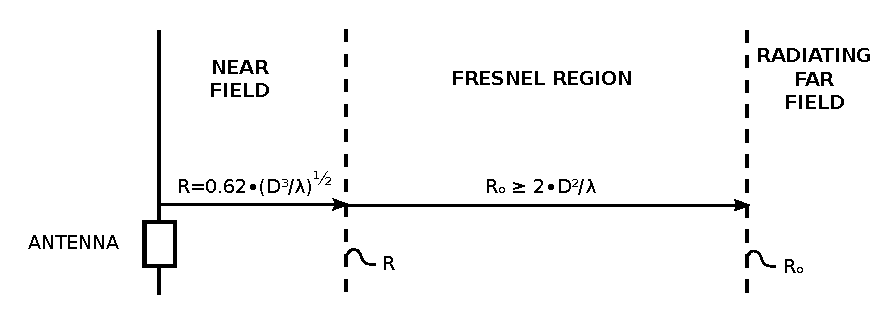
\includegraphics[width=0.9\textwidth]{./figs/02-state-of-the-art/FarNearFields-USP-4998112.pdf}
    \caption[\ac{em} Field for antennas larger than the wavelength of the radiation it emits]{\ac{em} Field for antennas larger than the wavelength of the radiation it emits~\cite{zerodamageFarFieldsVectorized1991}}. 
    \label{fig:fieldregionsbigantenna}
\end{figure}

For small antennas, shorter than half of the wavelength of the emitting radiation, the \emph{near-field} for \ac{rfid} applications is usually upper limited by $\lambda / 2\pi = 0.159\lambda$~\cite{nikitinOverviewFieldUHF2007a}.
Small antennas are used in \ac{lf} and \ac{hf} \ac{rfid} technologies.
For these technologies, which depend on the \emph{near-field} for mutual coupling, the limit of the reactive region is the theoretical limit for the read distance.
A delimitation of field regions for small antennas can be seen in figure~\ref{fig:fieldregionsshortantenna}.

\begin{figure}[!ht]
    \centering
    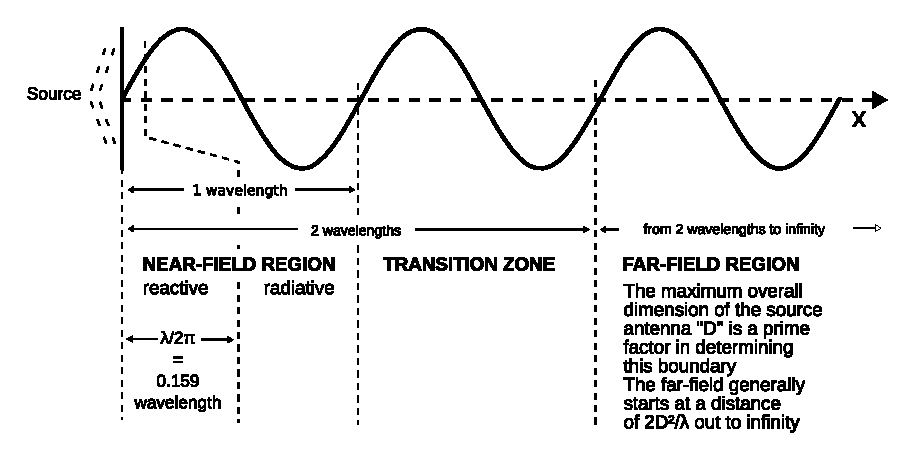
\includegraphics[width=0.9\textwidth]{./figs/02-state-of-the-art/Field_regions_for_typical_antennas_vector.pdf}
    \caption[Fields for antennas equal to, or shorter than, one-half wavelength of the radiation they emit]{Fields for antennas equal to, or shorter than, one-half wavelength of the radiation they emit~\cite{SafetyHealthTopics}} 
    \label{fig:fieldregionsshortantenna}
\end{figure}

\section{Tag} \label{sec:tag}

An \ac{rfid} tag, also called transponder, is a device that can store and transmit data to a compatible reader in a contactless manner using radio waves or electro-magnetic fields.

Tag cost is the main factor in long term return on investment in \ac{rfid} systems. It is one of the most important consideration when designing systems. After the initial investment in infrastructure, the expenses are mainly the acquisition of new tags.
The reduction of cost per tag is the central focus of manufacturers and what allows the technology to be competitive in the world of \ac{scm}.

At its simplest composition~\footnote{an inductive RC resonant tag used in anti-theft systems is considered an \ac{rfid} device, but is far from the requirements of modern \ac{rfid} paradigms}, a tag contains a microchip and an antenna, ilustrated on figure~\ref{fig:passivetag}.
Depending on the technology the tag architecture and operation varies.
Tags are characterized by their microchip, power source, memory characteristics and operating frequency. The following subsections will discussed these in detail.

\begin{figure}[!ht]
    \centering
    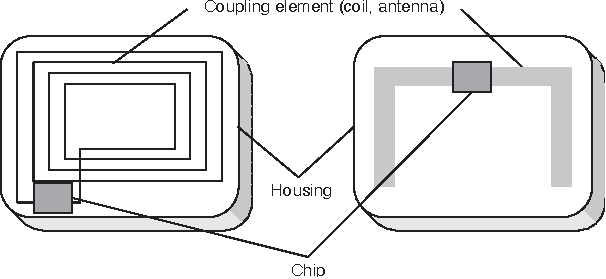
\includegraphics[width=0.65\textwidth]{./figs/02-state-of-the-art/tag.pdf}
    \caption[Components of a passive tag]{Components of a passive tag~\cite{finkenzellerRFIDHandbookFundamentals2003}} 
    \label{fig:passivetag}
\end{figure}

\subsection{Data Quantities}

In the contextualization of \ac{rfid} presented in section~\ref{sec:contextualization}, we discussed the concept of identification and how it can be as simple as World War II \ac{iff} systems. 
An unidentified aircraft presents, upon radar lightening, its identification as being friend or foe. In computing language this can be abstracted as true or false, or $1$ or $0$. This kind of systems does not exchange more than a bit of information, the smallest unit of information, that can represent only two states.
This type of transponders are called $1$-bit transponders. Despite the limitations, they are still widely used in surveillance and and anti-theft systems. Apparel retailers and other goods retailers have been using them for almost $6$ decades and are still well established nowadays. 
This dissertation requires the identification of more than $2$ types of objects, so the following content will jump over technical explanations of this type of transponder~\cite{finkenzellerRFIDHandbookFundamentals2003}. 

The type of transponder discussed through out this dissertation are n-bit transponders which use an electronic microchip as the data carrying device.
These transponders can transfer data in different methods and are currently used in a variety of standards all over the globe.

The following sections of this chapter will approach concepts that are required to understand systems using n-bit tags, specifically \acs{uhf}~\acs{rfid}.
For a deeper analysis of other \ac{rfid} systems refer to \emph{The RFID Handbook by Klaus Finkenzeller}~\cite{finkenzellerRFIDHandbookFundamentals2003}.

\subsection{Power Supply}

\subsubsection{Passive tags}

Passive tags are characterized for not having an on-board power source. 
Instead they use the power emitted from the reader antenna to energize themselves and transmit the stored data to the reader.
As such, tag-to-reader communication is always started by a reader, since it needs to energize the tag.

A few examples of state of the art passive \ac{uhf} tag inlays can be seen in figure~\ref{fig:alienAlienProductFamily2020}.
The simple constitution makes these tags robust, capable of withstanding corrosive chemicals such as acid and high temperatures~\footnote{The new Impinj M730 and M750 \ac{uhf} regular tags for item tagging sustains \ang{206}C for 1 minute and can retain data at \ang{125}C for 1 year~\cite[Tab. 18]{ImpinjM730M750}}.
These are the type of tags that underwent most technology advancements in the last decade in order to meet performance, compatibility and cost expectations that make mass deployment feasible for companies.

\begin{figure}[!ht]
    \centering
    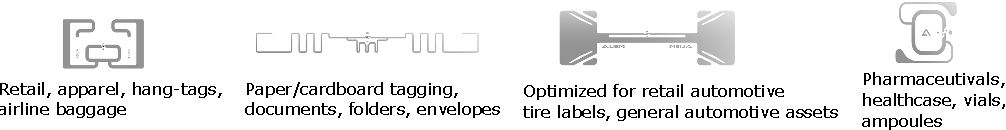
\includegraphics[width=\textwidth]{./figs/02-state-of-the-art/tag_examples.pdf}
    \caption[Selection of passive \ac{uhf} tag inlays for distinct applications from \textit{Alien Technology, LLC} 2020 Product Family]{Selection of passive \ac{uhf} tag inlays for distinct applications from \textit{Alien Technology, LLC} 2020 Product Family~\cite{alienAlienProductFamily2020}} 
    \label{fig:alienAlienProductFamily2020}
\end{figure}

\subsubsection{Active tags}

Active tags have on-board power source and use it to transmit data to the reader.
These type of tags do not need reader's emitted power for data transmission, therefore, in tag-to-reader communication, tags can either communicate first or be interrogated by a reader.
Usually, active tags stay in a low-power state (i.e.\ sleep) in the absence of interrogation by the reader. When a reader wants to interact with a tag, issues a wake up command. The tag transits out the low-power state and resolves the interrogation.
The \ac{rf} environment generated by systems with these type of tags has generally much lower \ac{rf} noise.

Since the presence of the reader is not necessary for data transmission, an active tag can broadcast its data, like a beacon, to its surrounding even in the absence of a reader. This is what is denominated as \emph{transmitter}.
Widely used for \ac{iot} applications as ``wireless computers'' to measure, process and transmit information about sensors, but out the scope of this dissertation. 

\begin{figure}[!ht]
    \centering
    \begin{subfigure}{.4\textwidth}
        \centering
        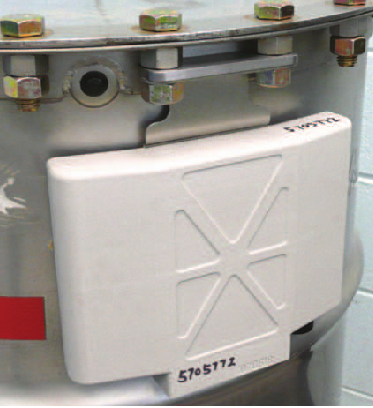
\includegraphics[width=.8\linewidth]{./figs/02-state-of-the-art/active_tag1.pdf}
        \caption{Tag mounted on Model 9975 drum}
        \label{fig:activetagsub1}
    \end{subfigure}
    \begin{subfigure}{.4\textwidth}
        \centering
        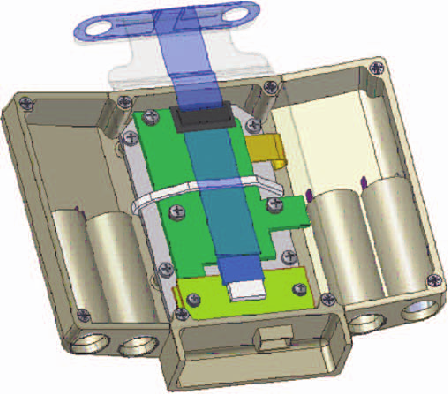
\includegraphics[width=0.95\linewidth]{./figs/02-state-of-the-art/active_tag2.pdf}
        \caption{Interior view of tag with metal back plate removed}
        \label{fig:activetagsub2}
    \end{subfigure}
    % Change caption
    \caption[\ac{us} Department of Energy prototype active tag with sensors for nuclear materials management working in $433.9MHz$ \ac{uhf} ISO band]{\ac{us} Department of Energy prototype active tag with sensors for nuclear materials management working in $433.9MHz$ \ac{uhf} ISO band~\cite{tsaiApplyingRFIDTechnology2008}} 
    \label{fig:activetag}
\end{figure}

\subsubsection{Semi-passive tags}

Semi-passive tags, also called \emph{semi-active} or \emph{battery assisted} tags, have on-board power source, but contrarily to active tags, it is only used for energizing the tag itself, thus, for transmitting its data, a semi-passive tag uses the reader's emitting power.

There are advantages of using these type of tags over passive ones.
Semi-passive tags do not use the reader signal to excite itself, so it can be read from further distances compared to passive tags. Because no time is needed to energize a semi-passive tag, it can also be read much faster than a passive one, making them useful for applications were the tag is in the reading zone for a short period of time (e.g.\ tolls on highways). Finally, this type of tag might also offer better readability in \ac{rf}-opaque and \ac{rf}-absorbent materials.

\begin{figure}[!ht]
    \centering
    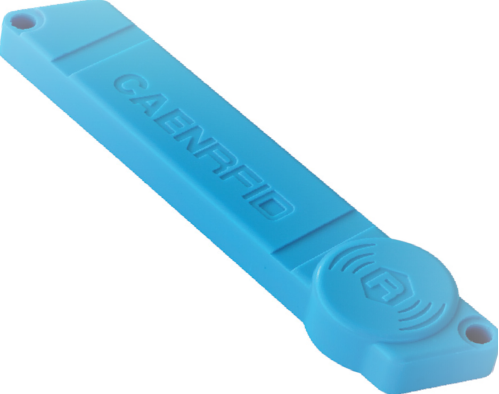
\includegraphics[width=0.3\textwidth]{./figs/02-state-of-the-art/semiactive_tag.pdf}
    \caption[\textit{CAEN RFID} A927Z semi-passive \ac{uhf} logger tag for temperature monitoring of sensitive products during transportation and storage]{\textit{CAEN RFID} A927Z semi-passive \ac{uhf} logger tag for temperature monitoring of sensitive products during transportation and storage~\cite{caenCaenA927ZTemp}} 
    \label{fig:semipassivetag}
\end{figure}

\subsection{Coupling}

We discussed in section~\ref{sec:em} how \ac{emf} behave throughout the space surrounding a transmitting antenna. Lets now understand how \ac{rfid} technologies take advantage of \acl{rf} to establish a communication channel between reader and tag.

Coupling in \ac{rfid} refers to the energy absorbed by a receiving antenna when a transmitting one is operating. 
It is a fundamental concept in \ac{rfid} communications and affects several aspects of a system including range, frequency and cost.
The coupling method and operating frequency are the defining parameters of technology categorization in \ac{rfid}, presented in section~\ref{sec:opfrequency} and used all over the world as a baseline to describe \ac{rfid} systems.

There are three types of coupling techniques: inductive, capacitive and backscatter. 
This dissertation focuses on passive tag systems operating in the \emph{remote-couple} (i.e.\ range from $1$cm to $100$cm) and \emph{long-range} (i.e further than $100$cm).
Capacitive coupling is only exploited for data transmission in \emph{close coupling systems} (i.e.\ range less than $1$cm), therefore this type of coupling technique will not be discussed.

\subsubsection{Inductive}

Inductive-coupling systems, also known as magnetic-coupling, use the \emph{near-field} magnetic component of the \ac{emf} to establish a mutual coupling between reader and tag.

The reader antenna coil generates a strong high frequency \ac{em} field. The variation of the magnetic flux excites the cross-section of the tag coil and induces a voltage.
Considering the wavelength of the frequency range used (< 135 kHz: 2400m, 13.58MHz: 22.1m) is several times greater than the distance between reader antenna and the transponder, we can treat it just like a simple inductive coupling system, just like a transformer.

This voltage is rectified and supplied to the tag circuitry.
The circuitry is actually designed to resonate at the transmission frequency of the reader. The resonance will generate high current in the reader, which produces the required field strength necessary for operation.

To transmit data from tag to reader, inductive systems use load modulation. The microchip changes de load on its coil in relation with the digital data to transmit. When a transponder, resonant at the transmission frequency of the reader, is placed in the reactive \emph{near-field} region, through mutual coupling, energy is drawn by the transponder, being detected by the reader as a voltage drop in the internal resistance of the reader through supply of current to the reader antenna.
An illustration of an inductive coupled load modulation \ac{rfid} system can be seen in figure~\ref{fig:loadmodulation}.

\begin{figure}[!ht]
    \centering
    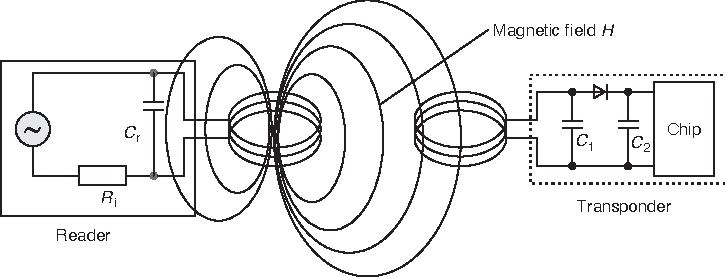
\includegraphics[width=0.9\textwidth]{./figs/02-state-of-the-art/loadmodulation.pdf}
    % Change caption
    \caption[Inductive coupled \ac{rfid} system overview]{Inductive coupled \ac{rfid} system overview~\cite{finkenzellerRFIDHandbookFundamentals2003}} 
    \label{fig:loadmodulation}
\end{figure}

This modulation method presents a fundamental problem. Due to weak coupling between antennas, there are voltage fluctuations at the antenna of the reader that are much higher than the fluctuations generated by the load modulation in the transceiver. This is a problem that usually appears in \ac{lf} \ac{rfid} systems. Detecting this slight voltages requires highly complicated circuitry which is undesirable.
Modern systems (e.g. $13.58$MHz \ac{hf} \ac{rfid}) use what is called: \emph{load modulation with subcarrier}. It uses the side bands created around the operating frequency ($f_T$) for the transmission of data. Switching the load resistor at a high elementary frequency ($f_s$), generates two spectral lines at a distance of $\pm f_s$ which contains the modulated signal. An illustration of this can be seen in figure~\ref{fig:loadmodulationsidebands}. The reader can demodulate and retrieve information that is carried in the sidebands of the two subcarrier sidebands, which are themselves created by the modulation of the subcarrier.

\begin{figure}[!ht]
    \centering
    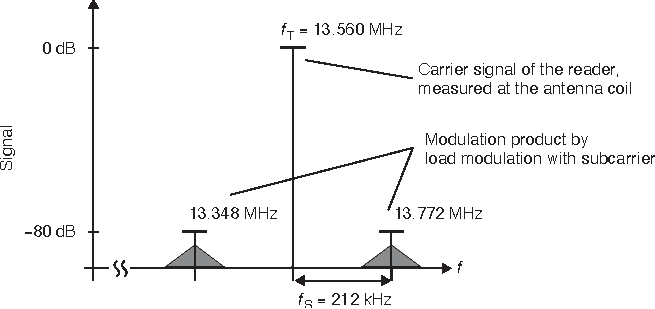
\includegraphics[width=0.7\textwidth]{./figs/02-state-of-the-art/loadmodulation_sidebands.pdf}
    \caption[Load modulation with subcarriers of a typical \ac{hf} \ac{rfid} system]{Load modulation with subcarriers of a typical \ac{hf} \ac{rfid} system~\cite{finkenzellerRFIDHandbookFundamentals2003}} 
    \label{fig:loadmodulationsidebands}
\end{figure}

Despite wide scale use and established global standardization, this type of coupling presents a few drawbacks. The reading distance is physically limited by the size of the reader antenna and the reactive \emph{near-field} boundary discussed throughout section~\ref{sec:em}. The shrinkage of tag size is also technically challenging due to the power emissions regulations and the dependence with the variation of the magnetic flux through the cross-section of the tag antenna coil, that excites the tag circuitry. The power consumption is also much higher than the next coupling technique we will look at, making it unsuitable for \emph{long-range systems}.

\subsubsection{Backscatter}

Backscatter coupling harvests energy from the \acp{emw}, transmitted by the reader antenna, to power the tag circuitry. It is mainly used in \emph{long-range systems} since it is the primarily coupling technique capable of operate in the \emph{far-field} region.
To transmit data back to the reader, the tag \textit{reflects} back some of the power as a modulated signal through what is called \emph{modulated reflection cross-section}.

\emph{Modulated reflection cross-section} operated by the same fundamental principles as the first \ac{rfid} system invented and presented in section~\ref{sec:contextualization}.
It is known from radar technologies that \acp{emw} are reflected by objects with dimensions greater than around half the wavelength of the wave.
The efficiency with which an object reflects \ac{emw} is described by its \emph{reflection cross-section}. Objects that are in resonance with the wave front that hits them, as is the case for antennas tuned to the appropriate frequency, have a particularly large \emph{reflection cross-section}.

The modulation of the \ac{rf} signal is created by changing the impedance viewed from the tag antenna, in similar manner to inductive coupling systems. 
Depicted in figure~\ref{fig:backscatter}, a load resistor, connected in parallel with the antenna, is switched on and off in time with the data stream to be transmitted.
The power reflected back changes in amplitude with the changing of impedance of the tag.
The reflected signal is picked by the reader antenna, decoupled using a \emph{directional coupler}, and finally demodulated~\cite{finkenzellerRFIDHandbookFundamentals2003, RFIDCouplingTechniques}.

\begin{figure}[!ht]
    \centering
    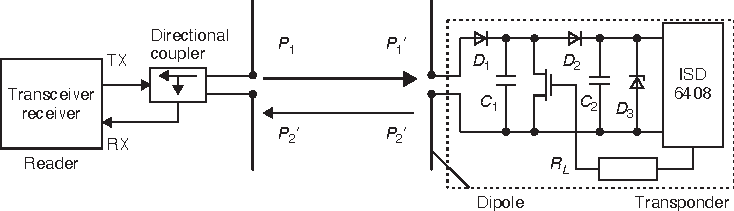
\includegraphics[width=0.9\textwidth]{./figs/02-state-of-the-art/backscatter.pdf}
    \caption[Passive backscatter RFID system]{Passive backscatter RFID system~\cite{finkenzellerRFIDHandbookFundamentals2003}} 
    \label{fig:backscatter}
\end{figure}

\subsection{\ac{rfid} Technologies} \label{sec:opfrequency}

When categorizing systems, the main aspect that defines \ac{rfid} technologies is the operating frequency.
In the previous sections we noticed a clear relation between operating frequency, through the wavelength, and system specifications like reading distance and data transfer speeds.
So, it is no accident that this spontaneous categorization happened. \ac{rfid} technologies tend to mature in a very clear path, being encompassed under use case specific standards with fixed operating frequencies carefully assigned by regulatory \ac{rf} authorities in each country. 
It is indeed a useful classification method to summarize a set of specifications that usually need to be established a priori in \ac{rfid} system design.

Being so, it is common in \ac{rfid} slang to name systems by the frequency band they operate in.
There are four preeminent frequency groups: \ac{lf}, \ac{hf}, \ac{uhf} and Microwave. \ac{uwb} \ac{rfid} technologies will not be discussed, being in early phases of technological development.
Each of the frequency groups presents characteristics inherent to their physical limitations that should be considered when choosing a technology.

\subsubsection{\acf{lf}}

\ac{lf} usually operates in the $125$KHz to $134$KHz frequency range, using passive tags through inductive coupling. Inherently, it has slow read speed and the reading range is limited to around $0.5m$. Despite the drawbacks, they have good behavior in metals and liquids and are the most mature technology, probably having the largest installed based system.
It is widely used in animal identification (ISO 11784/5~\cite{isoISO117841996, isoISO117851996}, ISO 14223~\cite{isoISO1422332018}), access control, logistics and data collection~\cite{isoISOIEC180002}, and automotive industry, in car ignition keys, to say a few.

\subsubsection{\acf{hf}}

\ac{hf} operates mostly around the $13.54$MHz frequency band. In same manner as \ac{lf}, it uses inductive coupling. The higher operating frequency allows faster data read speeds while maintaining semi-decent behavior in metals and liquids.
Widely used in smart cards~\cite{isoISOIEC156932, MIFARE} for all kinds of applications and is the basis of \ac{nfc} technology~\cite{isoISOIEC144434, isoISOIEC180003}. \ac{nfc} has been receiving a lot of attention. It is a global communication standard with a mature market (being roughly in any smartphone nowadays). This promoted big companies to invest in it, which began a wide scale manufacturing, resulting in the reduction of tag price (\$0.35 - \$10.00 per tag) and increase in system deployments.

\subsubsection{\acf{uhf}}

\ac{uhf} operates in the band of $315$MHz to $433$MHz using active tags~\cite{isoISOIEC180007}, and $860$MHz to $956$MHz using passive ones~\cite{isoISOIEC180006}. It is known for the promises it brings to \ac{scm} and logistics, being a cheap and affordable technology to wirelessly identify and track every item. It is mainly used in item tracking, but it can be adjusted for all kinds of applications. It uses backscatter coupling to transmit data between reader and tag. These frequencies present some drawbacks: poor behavior on liquid and metals is a big problem with passive tags; the allocation of the \ac{rf} spectrum differs between countries being a huge problem for global deployments. This thematic will be further discussed throughout this dissertation.

\subsubsection{Microwave}

Microwave typically operates at $2.45$GHz~\footnote{$5.8$GHz ISO standard was withdrawn}~\cite{isoISOIEC180004}, also called \emph{Industry, Scientific, and Medical (ISM)} band, accepted globally. Uses backscatter coupling with passive, semi-passive and active tags. It performs very poorly in the presence of metals and liquids.

\subsubsection{\ac{rf} Materials Performance}

\ac{rfid} technologies, operating in the different frequencies, perform differently in the presence of distinct materials.
Material can be: \acs{rf}-lucent, in that they are translucent to \acp{emw}; \acs{rf}-opaque, where \ac{emf} can not penetrate the material; and \acs{rf}-absorbent, in that it absorbs part of the \ac{emf} energy.
Concise information on \ac{rf} properties in different materials is presented in table~\ref{tab:rfproperties}.

\begin{table}[!htb]
    \centering
    \caption[\ac{rf} properties in different materials]{\ac{rf} properties in different materials~\cite{lahiriRFIDSourcebook2005}}
    \begin{tabular}{|l|l|l|l|l|}
    \hline
    \textbf{Material}     & \textbf{LF} & \textbf{HF} & \textbf{UHF} & \textbf{Microwave} \\ \hline
    Clothing              & RF-lucent   & RF-lucent   & RF-lucent    & RF-lucent          \\ \hline
    Dry wood              & RF-lucent   & RF-lucent   & RF-lucent    & RF-absorbent       \\ \hline
    Graphite              & RF-lucent   & RF-lucent   & RF-opaque    & RF-opaque          \\ \hline
    Liquids (some types)  & RF-lucent   & RF-lucent   & RF-absorbent & RF-absorbent       \\ \hline
    Metals                & RF-lucent   & RF-lucent   & RF-opaque    & RF-opaque          \\ \hline
    Motor oil             & RF-lucent   & RF-lucent   & RF-lucent    & RF-lucent          \\ \hline
    Paper products        & RF-lucent   & RF-lucent   & RF-lucent    & RF-lucent          \\ \hline
    Plastics (some types) & RF-lucent   & RF-lucent   & RF-lucent    & RF-lucent          \\ \hline
    Shampoo               & RF-lucent   & RF-lucent   & RF-absorbent & RF-absorbent       \\ \hline
    Water                 & RF-lucent   & RF-lucent   & RF-absorbent & RF-absorbent       \\ \hline
    Wet wood              & RF-lucent   & RF-lucent   & RF-absorbent & RF-absorbent       \\ \hline
    \end{tabular}
    \label{tab:rfproperties}
\end{table}

There is a big market around single purpose tags for materials with poor \ac{rf} performance. 
An informed decision must be made when selecting tags for systems dealing with materials portraying these characteristics.

\section{Reader} \label{sec:reader}

A reader is a device that can read from and write data to compatible \ac{rfid} tags. It is responsible for sending and receiving \ac{rf} signals to and from tags.
If we strip down all the features modern readers offer, we can isolate three main components: \ac{rf} front-end, processor, communication interface. % not features - architectural blocks (corrigir)

The \ac{rf} front-end interfaces with the reader antenna. 
It is responsible for transmitting power and clock cycle via the antenna to tags in the reading zone, and demodulate \ac{rf} signals received from tags to be further handled by the processor. 
Readers must adhere to \ac{rf} modulation requirements and \ac{eirp} regulations if they want to be approved and commercialized. This fact promotes the implementation of the front-end by a dedicated transceiver microchip and complementary electronics, which is usually chosen. There are also efforts in implementing the \ac{rf} front-end in \acp{fpga}, which might change this paradigm in the next few years~\cite{hugomanueloliveirademirandaSistemasRFIDUHF2015}.

The processor is responsible for all logic necessary in the reader. It often comes with other complementary components like memory and dedicated \acp{ic} for specific tasks. Readers differ in architecture design between manufacturers, but the processor must at least implement the reader protocol to communicate with compatible tags. This includes decoding and error checking of the analog signals from the \ac{rf} front-end, a controller interface to allow external entities to communicate with it, to transfer stored data, issue commands, accept commands and control the reader functions.

Communication interface is the component that provides communication instruction to a reader which allows external entities to interact with it.
It usually comes inside microprocessors and microcontrollers \acp{ic}. It is usually seen in commercial readers as serial communication interface or ethernet.

Commercial readers come in a variety of types which are suited for different applications.
The most common are stationary readers. Also called, \emph{fixed} readers, they are what the name implies, used for making fixed reading zones. They also can be mounted on forklifts and inside of trucks.
Other types are handheld readers, for a portable reading device and \ac{rfid} printers which are used to print smart labels.

\section{Reader Antenna} \label{sec:antenna}

A reader communicates with tags through its antenna. 
Antennas are responsible for converting guided \acp{cw} in radiating \ac{emw} and vice-versa.
It will only be covered radiating antenna theory for it is what is necessary to follow this dissertation.

In handheld readers, the antenna is generally integrated into the device. In stationary readers is most commonly found as a separate device attached to an antenna port of the reader by means of a cable.
There are different groups of antenna designs: antennas composed of a wire, which encompass the dipole, monopole and loop antennas; constituted of an opening, like the horn and cavity backed slot antennas % rever isto
; and printed circuit antennas like path antennas, commonly used in \acs{uhf}~\acs{rfid}.

Evaluating antennas for \ac{rfid} systems can be done through the parameters specified by the manufacturer, a few rules of thumb and engineering sensibility.
At \ac{uhf} we can control the direction of waves and other parameters, and thus improve the readability of tags.

\subsection{Radiation pattern}

An important parameter in antenna selection is the radiation pattern. 
Radiation pattern is the mathematical description or representation of the radiation properties of the antenna as a function of space coordinates.
The radiation pattern illustrates the regions where the antenna's energy is most effective.
In \ac{rfid} is usually called the footprint of the antenna and determines the read zone.
Manufacturers usually provide the radiation patterns for \ac{rfid} antennas in the datasheet.

Different antenna designs radiate with different patterns. These radiation patterns are classified in three main classes: isotropic, directional and omnidirectional.
For \acs{uhf}~\acs{rfid}, directional antennas are really useful since it is possible to maximize directivity, that is, how well the radiation emitted is concentrated in a single direction. This increases reading distances and defines boundaries in reading zones. \acs{uhf}~\acs{rfid} directional antennas are commonly patch antennas, also called \emph{microstrip} or \emph{planar antennas}. They consist of rectangular metal foil or a plate mounted on a substrate such as Teflon or FR-4 (i.e.\ woven fiberglass cloth with an epoxy resin binder).

Is also important, when designing \ac{rfid} systems, to have notion of the deformations that occur in the radiation patterns.
\emph{Multi-path} phenomena - the reflection of \ac{emw} in \ac{rf}-opaque objects which causes waves to be scattered and arrive back at the reader in different paths and times - results in \emph{phase} shifts leading to constructive and destructive interference.
This creates protrusions and dead zones that will inevitably exist in most \acs{uhf}~\acs{rfid} and microwave systems deployments. 

%\subsection{Gain}

%They gain parameter is also "important" when selecting an \ac{rfid} antenna.
%It characterizes the performance of the antenna by mathematically describing how well it converts input power into radio waves radiated in a specified direction. It relates directivity and efficiency.

\subsection{Polarization}

Antennas radiate \ac{emw} into surrounding space.
Polarization is the direction of oscillation of the \ac{emw} and has a great importance in tag readability.

\acp{emw} behave similarly to a wave of water. When a wave from a source, like a boat, reaches a buoy, the buoy moves mostly up and down.
Analogously, \ac{emw} moves electrons in the plane perpendicular to the direction of propagation. The direction in which the field points, determines the polarization of the \ac{emw}.
Unlike water waves, \acp{emw} are not influenced by gravity, so the electric field can point in any direction in the plane perpendicular to the direction of propagation, and so have different polarizations~\cite{dobkinRFRFIDSecond2012}.

The main types of polarization are known as linear and circular. Both types derive from the elliptical polarization, being linear and circular special cases of such.

\subsubsection{Linear polarization}

Linear polarized antenna emanate \acp{emw} in a linear pattern, that is, emits \ac{emw} with only one field of energy.

These antennas have a narrower radiation beam with better directivity compared to circular polarized antennas. This results in longer reading distances and well-defined reading regions, which are essential to good \ac{rfid} system design.

These advantages can sometimes fall short to the disadvantages. Linear antennas are sensitive to tag orientation with respect to its polarization direction. 
\ac{rfid} tag antennas are usually dipoles constituted of narrow metal traces aligned in one direction. If the electric field is directed along the traces, it can push electrons back and forth inducing the voltage necessary to energize the tag \ac{ic}. If the electric field is directed perpendicular to the trace axis, it moves electrons across the diameter of the trance, producing negligible current, insufficient to power the tag \ac{ic}.
Linear antennas are generally used in applications where tag orientation is fixed and predictable, or in conjunction with other complementary linear antennas.

\subsubsection{Circular polarization}

Circular polarized antennas solve, to certain degree, the orientation dependence problem with detriment of reading distance and a wider radiation beam.
These antennas produce two energy fields that are equal in amplitude and magnitude, with a phase difference of $90^\circ$ between them. This results in the electric field vector to be seen as helix like trace, a circular motion propagating through space. 

Because the nature of circular polarized antennas, they are to a certain extent, unaffected by tag orientation.
A circularly polarized \ac{emw} interacts with the linear antenna of a tag, tilted at any angle within the plane perpendicular to the axis of propagation, but in every case only half the transmitted power can be received.
Good antenna design in tags can modestly improve energy harvesting performance, e.g.\ incorporate two dipole antennas on the tag directed orthogonally to one another or physically larger bow-tie antenna designs.

These antennas are widely used in passive \acs{uhf}~\acs{rfid}, specially in \ac{rf} environment with high degree of \ac{rf} reflectance, like due to presence of metals.

% Edgar e Eu: ficava bem uma ilustração das possiveis orientações entre reader e tag. Adicionar umas imagens na section do Reader e isso

In the next chapter, I will introduce GS1 and their EPCGlobal Architecture Framework, used in \ac{scm} and logistics across the world and their close realtion with \ac{uhf} \ac{rfid}.  

\cleardoublepage